\documentclass{standalone}
\usepackage{tikz}
\usetikzlibrary{patterns, positioning}


\begin{document}
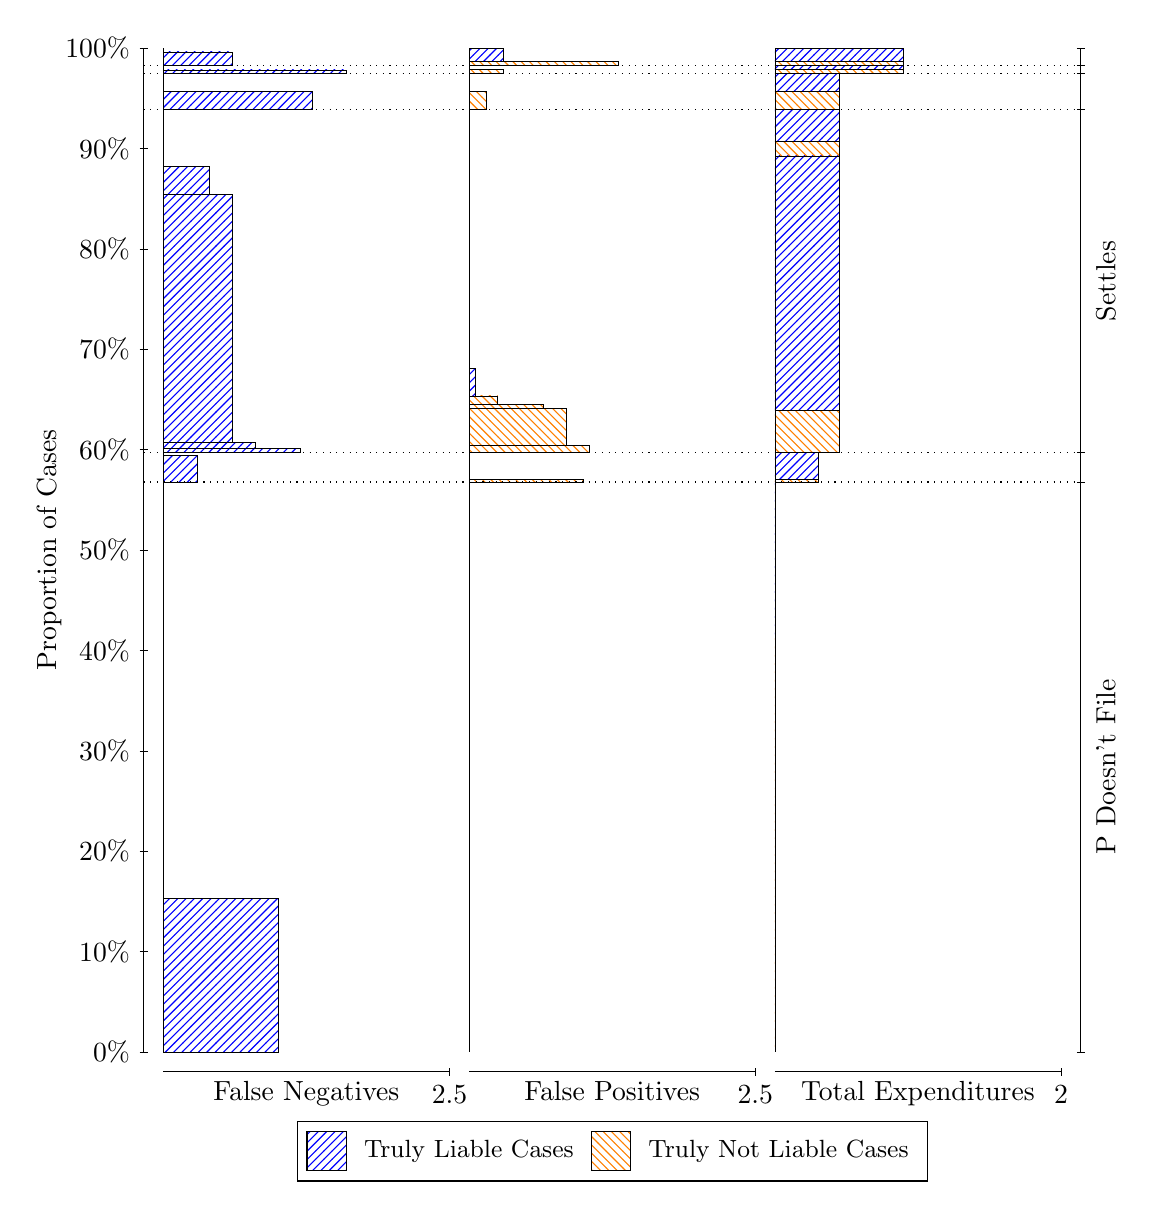
\begin{tikzpicture}
\draw[black, very thin] (1.5,1.75) -- (1.5,14.5);
\node[rotate=90, text=black, anchor=center] at (0.3, 8.125) {Proportion of Cases};
\draw[black, very thin] (1.45,1.75) -- (1.55,1.75);
\node[text=black, anchor=east] at (1.45, 1.75) {0\%};
\draw[black, very thin] (1.45,3.025) -- (1.55,3.025);
\node[text=black, anchor=east] at (1.45, 3.025) {10\%};
\draw[black, very thin] (1.45,4.3) -- (1.55,4.3);
\node[text=black, anchor=east] at (1.45, 4.3) {20\%};
\draw[black, very thin] (1.45,5.575) -- (1.55,5.575);
\node[text=black, anchor=east] at (1.45, 5.575) {30\%};
\draw[black, very thin] (1.45,6.85) -- (1.55,6.85);
\node[text=black, anchor=east] at (1.45, 6.85) {40\%};
\draw[black, very thin] (1.45,8.125) -- (1.55,8.125);
\node[text=black, anchor=east] at (1.45, 8.125) {50\%};
\draw[black, very thin] (1.45,9.4) -- (1.55,9.4);
\node[text=black, anchor=east] at (1.45, 9.4) {60\%};
\draw[black, very thin] (1.45,10.675) -- (1.55,10.675);
\node[text=black, anchor=east] at (1.45, 10.675) {70\%};
\draw[black, very thin] (1.45,11.95) -- (1.55,11.95);
\node[text=black, anchor=east] at (1.45, 11.95) {80\%};
\draw[black, very thin] (1.45,13.225) -- (1.55,13.225);
\node[text=black, anchor=east] at (1.45, 13.225) {90\%};
\draw[black, very thin] (1.45,14.5) -- (1.55,14.5);
\node[text=black, anchor=east] at (1.45, 14.5) {100\%};

\draw[black, very thin] (13.4,1.75) -- (13.4,14.5);
\draw[black, very thin] (13.35,1.75) -- (13.45,1.75);
\node[anchor=west] at (13.35, 1.75) {};
\draw[black, very thin] (13.35,8.9882) -- (13.45,8.9882);
\node[anchor=west] at (13.35, 8.9882) {};
\draw[black, very thin] (13.35,9.3652) -- (13.45,9.3652);
\node[anchor=west] at (13.35, 9.3652) {};
\draw[black, very thin] (13.35,13.718) -- (13.45,13.718);
\node[anchor=west] at (13.35, 13.718) {};
\draw[black, very thin] (13.35,14.173) -- (13.45,14.173);
\node[anchor=west] at (13.35, 14.173) {};
\draw[black, very thin] (13.35,14.283) -- (13.45,14.283);
\node[anchor=west] at (13.35, 14.283) {};
\draw[black, very thin] (13.35,14.5) -- (13.45,14.5);
\node[anchor=west] at (13.35, 14.5) {};

\draw[black, very thin, pattern color=blue, pattern=north east lines] (1.75,1.75) rectangle (3.2033,3.7034);
\draw[black, very thin, pattern color=orange, pattern=north west lines] (1.75,3.7034) rectangle (1.75,8.9882);
\draw[black, very thin, pattern color=blue, pattern=north east lines] (1.75,8.9882) rectangle (2.186,9.3298);
\draw[black, very thin, pattern color=orange, pattern=north west lines] (1.75,9.3298) rectangle (1.75,9.3652);
\draw[black, very thin, pattern color=blue, pattern=north east lines] (1.75,9.3652) rectangle (3.494,9.4111);
\draw[black, very thin, pattern color=blue, pattern=north east lines] (1.75,9.4111) rectangle (2.9127,9.4924);
\draw[black, very thin, pattern color=blue, pattern=north east lines] (1.75,9.4924) rectangle (2.622,12.646);
\draw[black, very thin, pattern color=blue, pattern=north east lines] (1.75,12.646) rectangle (2.3313,13.001);
\draw[black, very thin, pattern color=orange, pattern=north west lines] (1.75,13.001) rectangle (1.75,13.718);
\draw[black, very thin, pattern color=blue, pattern=north east lines] (1.75,13.718) rectangle (3.6393,13.945);
\draw[black, very thin, pattern color=orange, pattern=north west lines] (1.75,13.945) rectangle (1.75,14.173);
\draw[black, very thin, pattern color=blue, pattern=north east lines] (1.75,14.173) rectangle (4.0753,14.223);
\draw[black, very thin, pattern color=orange, pattern=north west lines] (1.75,14.223) rectangle (1.75,14.283);
\draw[black, very thin, pattern color=blue, pattern=north east lines] (1.75,14.283) rectangle (2.622,14.45);
\draw[black, very thin, pattern color=orange, pattern=north west lines] (1.75,14.45) rectangle (1.75,14.5);
\draw[black, very thin, pattern color=orange, pattern=north west lines] (5.6333,1.75) rectangle (5.6333,7.0348);
\draw[black, very thin, pattern color=blue, pattern=north east lines] (5.6333,7.0348) rectangle (5.6333,8.9882);
\draw[black, very thin, pattern color=orange, pattern=north west lines] (5.6333,8.9882) rectangle (7.0867,9.0235);
\draw[black, very thin, pattern color=blue, pattern=north east lines] (5.6333,9.0235) rectangle (5.6333,9.3652);
\draw[black, very thin, pattern color=orange, pattern=north west lines] (5.6333,9.3652) rectangle (7.1593,9.4488);
\draw[black, very thin, pattern color=orange, pattern=north west lines] (5.6333,9.4488) rectangle (6.8687,9.9249);
\draw[black, very thin, pattern color=orange, pattern=north west lines] (5.6333,9.9249) rectangle (6.578,9.9778);
\draw[black, very thin, pattern color=orange, pattern=north west lines] (5.6333,9.9778) rectangle (5.9967,10.082);
\draw[black, very thin, pattern color=blue, pattern=north east lines] (5.6333,10.082) rectangle (5.706,10.437);
\draw[black, very thin, pattern color=blue, pattern=north east lines] (5.6333,10.437) rectangle (5.6333,13.718);
\draw[black, very thin, pattern color=orange, pattern=north west lines] (5.6333,13.718) rectangle (5.8513,13.945);
\draw[black, very thin, pattern color=blue, pattern=north east lines] (5.6333,13.945) rectangle (5.6333,14.173);
\draw[black, very thin, pattern color=orange, pattern=north west lines] (5.6333,14.173) rectangle (6.0693,14.233);
\draw[black, very thin, pattern color=blue, pattern=north east lines] (5.6333,14.233) rectangle (5.6333,14.283);
\draw[black, very thin, pattern color=orange, pattern=north west lines] (5.6333,14.283) rectangle (7.5227,14.334);
\draw[black, very thin, pattern color=blue, pattern=north east lines] (5.6333,14.334) rectangle (6.0693,14.5);
\draw[black, very thin, pattern color=orange, pattern=north west lines] (9.5167,1.75) rectangle (9.5167,7.0348);
\draw[black, very thin, pattern color=blue, pattern=north east lines] (9.5167,7.0348) rectangle (9.5167,8.9882);
\draw[black, very thin, pattern color=orange, pattern=north west lines] (9.5167,8.9882) rectangle (10.062,9.0235);
\draw[black, very thin, pattern color=blue, pattern=north east lines] (9.5167,9.0235) rectangle (10.062,9.3652);
\draw[black, very thin, pattern color=orange, pattern=north west lines] (9.5167,9.3652) rectangle (10.334,9.8942);
\draw[black, very thin, pattern color=blue, pattern=north east lines] (9.5167,9.8942) rectangle (10.334,13.129);
\draw[black, very thin, pattern color=orange, pattern=north west lines] (9.5167,13.129) rectangle (10.334,13.317);
\draw[black, very thin, pattern color=blue, pattern=north east lines] (9.5167,13.317) rectangle (10.334,13.718);
\draw[black, very thin, pattern color=orange, pattern=north west lines] (9.5167,13.718) rectangle (10.334,13.945);
\draw[black, very thin, pattern color=blue, pattern=north east lines] (9.5167,13.945) rectangle (10.334,14.173);
\draw[black, very thin, pattern color=orange, pattern=north west lines] (9.5167,14.173) rectangle (11.152,14.233);
\draw[black, very thin, pattern color=blue, pattern=north east lines] (9.5167,14.233) rectangle (11.152,14.283);
\draw[black, very thin, pattern color=orange, pattern=north west lines] (9.5167,14.283) rectangle (11.152,14.334);
\draw[black, very thin, pattern color=blue, pattern=north east lines] (9.5167,14.334) rectangle (11.152,14.5);
\draw[black, dotted] (1.5,8.9882) -- (13.4,8.9882);
\draw[black, dotted] (1.5,9.3652) -- (13.4,9.3652);
\draw[black, dotted] (1.5,13.718) -- (13.4,13.718);
\draw[black, dotted] (1.5,14.173) -- (13.4,14.173);
\draw[black, dotted] (1.5,14.283) -- (13.4,14.283);
\draw[black, very thin] (1.75,1.5) -- (5.3833,1.5);
\node[text=black, anchor=north] at (3.5667, 1.5) {False Negatives};
\draw[black, very thin] (5.3833,1.45) -- (5.3833,1.55);
\node[text=black, anchor=north] at (5.3833, 1.45) {2.5};

\draw[black, very thin] (5.6333,1.5) -- (9.2667,1.5);
\node[text=black, anchor=north] at (7.45, 1.5) {False Positives};
\draw[black, very thin] (9.2667,1.45) -- (9.2667,1.55);
\node[text=black, anchor=north] at (9.2667, 1.45) {2.5};

\draw[black, very thin] (9.5167,1.5) -- (13.15,1.5);
\node[text=black, anchor=north] at (11.333, 1.5) {Total Expenditures};
\draw[black, very thin] (13.15,1.45) -- (13.15,1.55);
\node[text=black, anchor=north] at (13.15, 1.45) {2};

\node[text=black, centered, rotate=90] at (13.72, 5.3691) {P Doesn't File};

\node[text=black, centered, rotate=90] at (13.72, 11.541) {Settles};




\draw (7.449999999999999,1.5) node[draw=none] (baseCoordinate) {};
\begin{scope}[align=center]
        \matrix[scale=0.5, draw=black, below=0.5cm of baseCoordinate, nodes={draw}, column sep=0.1cm]{
            \node[rectangle, draw, minimum width=0.5cm, minimum height=0.5cm, pattern color=blue, pattern=north east lines] {}; &
            \node[draw=none, font=\small, text=black] (B) {Truly Liable Cases}; &
            \node[rectangle, draw, minimum width=0.5cm, minimum height=0.5cm, pattern color=orange, pattern=north west lines] {}; &
            \node[draw=none, font=\small, text=black] (B) {Truly Not Liable Cases}; \\
            };
\end{scope}

\end{tikzpicture}
\end{document}